% This is samplepaper.tex, a sample chapter demonstrating the
% LLNCS macro package for Springer Computer Science proceedings;
% Version 2.21 of 2022/01/12
%
\documentclass[runningheads]{llncs}
%
\usepackage[T1]{fontenc}
% T1 fonts will be used to generate the final print and online PDFs,
% so please use T1 fonts in your manuscript whenever possible.
% Other font encondings may result in incorrect characters.
%
\usepackage{graphicx}
\usepackage{hyperref}
\usepackage{subfig}
\usepackage{booktabs}
\usepackage{amsmath}
\usepackage{bm}
\usepackage{dsfont}
\usepackage{algorithm}
\usepackage{algorithmic}
\usepackage{todonotes}
\usepackage{svg}

% Revision markup: changed or new text is red (xcolor is loaded by todonotes).
\newcommand{\rev}[1]{\textcolor{red}{#1}}

%
\begin{document}
%

\title{Energy-Efficient Flocking in Self-Organized Robot Swarms}
%

\titlerunning{Emergent Energy-Efficient Flocking}
% If the paper title is too long for the running head, you can set
% an abbreviated paper title here
%
\author{
Lilly Schwarzenbach\inst{1} \and
Sina Mahdavi\inst{2} \and
%Dushyant Singh\inst{1} \and
%Peter Klapwijk\inst{1} \and
Georges Jetti\inst{2}\orcidID{0009-0007-9682-4838} \and
Michael Khayyat\inst{2}\orcidID{0000-0002-1718-4198} \and
Francesco Braghin\inst{2}\orcidID{0000-0002-0476-4118} \and
Eliseo Ferrante\inst{1,3}\orcidID{0000-0002-2213-8356}}

%
\authorrunning{L.Schwarzenbach et al.}
% First names are abbreviated in the running head.
% If there are more than two authors, 'et al.' is used.
%
\institute{ Vrije Universiteit Amsterdam, Amsterdam, The Netherlands\\
\email{l.m.schwarzenbach@vu.nl}\and
Politecnico di Milano, Milan, Italy \and
New York University Abu Dhabi, Abu Dhabi, United Arab Emirates
}

\index{Schwarzenbach, Lilly}
\index{Mahdavi, Sina}
%\index{Singh, Dushyant}
%\index{Klapwijk, Peter}
\index{Jetti, Georges}
\index{Khayyat, Michael}
\index{Braghin, Francesco}
\index{Ferrante, Eliseo}
%
\maketitle              % typeset the header of the contribution
%
\begin{abstract} % 150-250 words

Groups of natural agents such as flocks of birds preserve energy by changing positions and thereby taking turns being exposed to the wind. We evolve an energy-aware controller for decentralized, memoryless, communication-free agents in a 2D environment. Our results show that being aware of neighbours' range and bearing, a digital compass and the battery level is enough to produce emergent reconfigurations akin to those observed in natural groups: in a swarm of 20 robots, the robot at the exposed front changes about ten times per minute, almost five times as often as in a traditional flocking baseline model.  \rev{On seven real robots, the evolved controller also shares the exposed front among the robots much more evenly than the baseline, as in simulation.}
We validate our model in simulation and real Thymio-II robots. In simulation with 20 robots, the evolved controller travels more than twice as far as the baseline before the first robot runs out of battery, while also retaining more battery. This advantage depends on swarm size: it appears only from about 13 robots upwards, and in small swarms the baseline performs better.

\end{abstract}
%
%
%
\section{Introduction}
One of the fundamental behaviours in robot swarms is that of collective motion, allowing a group of robots to move in an aligned fashion as a group\cite{vicsek-col-motion}. This offers numerous benefits, such as enhanced foraging \cite{couzin2005effective}, predator evasion \cite{olson2013predator}, efficient navigation \cite{couzin2005effective}, and improved hydrodynamic and aerodynamic performance \cite{beaver2021overview}.

However, animals and robots share a central limitation: Their movement is limited by the amount of energy at their disposal. Moving costs energy. Animals need to rest and feed to recharge; robots need to charge at a charging station or have their batteries changed. However, these activities cost time and in the case of robots, may require human intervention which is inconvenient especially in environments that are less accessible to humans such as cave systems, aerial or underwater inspection systems. It is therefore paramount to save energy wherever possible. For this purpose, we take inspiration from animals that have already developed energy-efficient behaviours such as bird flocks, fish schools, and insect colonies. They have a few things in common: They are fully decentralised, interactions are purely local, there are no explicit leaders, and there is no explicit communication. These assumptions are in line with those made by swarm robotics, which is known to produce scalable and cost-effective solutions\cite{Brambilla2013,Dorigo2021,Debie2023,FariaDias2021}. Therefore, it is only natural that researchers look to natural collective systems for understanding and design inspiration for swarm robotics applications\cite{Andersson2004,Voelkl2017,Mirzaeinia2020,Hassanalian2022,Beaumont2024,Friman2024}.

Previous work has identified dynamic reconfiguration as one of the key factors contributing to the improved aerodynamic performance in collective navigation\cite{beaver2021overview}, for example through heart-rate monitoring showing pelicans expend less energy flying in formation~\cite{weimerskirch2001} and by flight-path reconstructions showing ibis actively phase their wingbeats to exploit each other's upwash~\cite{portugal2014}. If the agents stay in the same positions throughout their journey, environmental effects remain unevenly distributed. In the case of migratory birds, the front positions are more energy-draining. By periodically changing positions, this energy drain can be distributed among agents and the individual agents lose less energy. Using this strategy, migratory birds save about 11-71\% energy depending on their position within the flock, while the flock itself can extend its flight range by up to 44.6\%~\cite{Voelkl2017,Mirzaeinia2020,Beaumont2024}. Similar energy savings from collective movement have also been reported in schooling fish~\cite{Zhang2024}. Human cycling pelotons have also been reported to employ similar strategies~\cite{Blocken2018}.

Although there is evidence for the importance o this reconfiguration behaviour, the literature in swarm robotics has considered energy efficiency and formation reconfiguration in isolation and not together with the exception of~\cite{mahdavi2026energy}, which we extend and further validate here.

Energy efficiency has been addressed in multiple ways in swarm robotics. Among other approaches, energy has been proposed as a proxy for a reward rather than a physical property which would cause the robots to fail~\cite{Elfwing2005,Weel2012,Haasdijk2013}. Another approach shows that using energy levels allows response-threshold policies to improve efficiency in self-assignment to either foraging or resting~\cite{Wenguo2007}. Other studies have proposed to tackle energy efficiency by optimising the hardware and the use of perception and communication~\cite{Yasin2021,Zhang2023,Ren2024}.

Formation reconfiguration is an active field in multi-robot systems but has not been widely explored under the more stringent requirements of swarm robotics. The v-shape common in flocks of birds specifically has been targeted in multiple works.
Yang et al. (2016)\cite{Yang2016} use MPC and achieve V-formation by optimizing over velocity matching between agents, clear view, and upwash benefit, in both centralized and decentralized frameworks. Roy et al. (2020)\cite{Roy2020} optimize a similar cost function and propose a learning based framework that combines MPC with DNC as a teacher-learner pair. Although these works were able to achieve the V-shaped flocking pattern using simple local rules, dynamic formation reconfiguration is missing from them. In addition, they required full knowledge of the aerodynamic landscape. Instead, a greedy leading/trailing replacement heuristic was proposed by Mirzaeinia et al. (2019)\cite{Mirzaeinia2019} to achieve dynamic formation reconfiguration using battery thresholds. Then, Liu et. al. (2024)\cite{Liu2024}\cite{2Liu2024} frame the same issue as an optimization problem but require the energetic cost of the positions as input. However, both works assumed particular fixed patterns, such as the V-formation, and solved dynamic position assignment within the confines of these formations. Also, they took advantage of global communication between members.

In this work, we address the problem of energy-efficient collective motion by evolving a controller for simple, memory-less robots in a 2D environment with uniform wind. The wind as well as the motion drains the battery and the group can only move while all of the robots still have battery.
We use an existing evolutionary swarm robotics framework first proposed in~\cite{vandiggelen2025emergentheterogeneousswarmcontrol}. Our contribution lies in applying this framework to a problem that has only been studied by~\cite{mahdavi2026energy} for far: Using only range and bearing sensors and a battery monitoring sensor, travel as far as possible as a group. The robots cannot sense the wind that contributes to the battery being drained nor do they have any information about the state of the other robots. We show that this is enough for dynamic reconfiguration to emerge and this strategy allows the group to travel further than a traditional flocking baseline model in line with the findings in~\cite{mahdavi2026energy}. We extend~\cite{mahdavi2026energy} by evolving the controller with a two-stage curriculum instead of using three stages. Additionally, we validate our findings on real robots. we quantify the reconfiguration with leadership metrics from studies of bird flocks. We also show that the advantage depends on the size of the swarm: controllers evolved with 20 robots outperform the baseline only in large swarms.  


This paper is organised as follows: Section~\ref{sec:methodology} presents the methodology and metrics, Section~\ref{sec:EXp_Setup} introduces the simulation environment and the setup for the real robot experiments as well as the model of the battery drainage. Subsequently, Section~\ref{sec:Exp:Results} presents our findings and finally, Section~\ref{sec:Conclusion} summarises our findings and draws conclusions from them.


\section{Methodology}
\label{sec:methodology}
The methodology is heavily based on the framework presented in~\cite{mahdavi2026energy} which in turn bases its methodology on~\cite{vandiggelen2025emergentheterogeneousswarmcontrol}. In both works as well as our own, every robot is equipped with a neural controller. The weights of the controller are updated by Hebbian learning rules which are learned through an evolutionary algorithm. All evolutionary and simulated validation experiments are performed in a 2D kinematic Python simulator.
The full workflow is depicted in Figure~\ref{fig:ES_overview}.

% CHECK: if ES_layout.png still shows the old three-stage pipeline, replace it with
% figures/method_pipeline (upload figures/method_pipeline.pdf from the repo).
\begin{figure}[t]
\centering
\includegraphics[width=1\textwidth]{Images/Methodology/ES_layout.png}
\caption{\textbf{Overview of the Methodology.}
    Our setup comprises a swarm with robots, each equipped with a neural network controller. Each swarm shares one set of Hebbian learning rules, which are learned by the CMA-ES algorithm through evolution. The robots are simulated in the windy arena for fitness calculation.} \label{fig:ES_overview}
\end{figure}

\subsection{Individual Robot Neural Controller}
We consider differential-drive ground robots modeling Thymio-II robots, the hardware platform used for the real world experiments. Their locomotion capabilities are regulated by forward velocity $v_i$ and angular velocity $\omega_i$.

\begin{figure}[t]
  \centering
  \subfloat[Bearing\label{fig:bearing}]{
    \begin{minipage}[t]{0.35\textwidth}
       \centering
      \includegraphics[width=0.7\linewidth]{Images/Methodology/quadrants.png}
    \end{minipage}
  }
  \subfloat[Range\label{fig:range}]{
    \begin{minipage}[t]{0.35\textwidth}
      \centering
      \includegraphics[width=0.7\linewidth]{Images/Methodology/quadrants_range.png}
    \end{minipage}
  }
  \caption{Sensing capabilities of the individual robots.}
  \label{fig:quadrants}
\end{figure}

We assume the robots can perceive neighbours only when they are within their sensing radius $R$ (in our experiments $R=2.01$\,m). The circle described by this radius is then divided into four quadrants $q \in [1,2,3,4]$, centred on the robot's front, left, back and right (Figure~\ref{fig:quadrants}). Instead of considering all neighbours, the robot only considers the nearest neighbour in each quadrant and knows that neighbour's distance, $d_q \in [0, R]$, and bearing, $\psi_q \in [0, \pi/2]$. In addition, the robot is aware of its battery-level, i.e. the percentage of battery remaining, $B_0 \in [0, 100]$. Furthermore, the robot also has a digital compass, $\theta_0 \in (-\pi, \pi]$, giving it an approximate task direction context. All sensor information is assumed to be noise-free in simulation while they are procured from a motion-capture system for the hardware validation (Section~\ref{sec:EXp_Setup}).

Each robot runs a 10-10-10-2 Multi-Layer Perceptron (MLP) with ReLU hidden layers and tanh outputs. The inputs to its neural network are the readings from the four quadrants, i.e. the distance and bearing of the nearest neighbour in that quadrant ($d^i_q, \psi^i_q$), as well as its battery level ($B^i_0$) and its heading ($\theta^i_0$). When the robot does not perceive any neighbours, its sensor readings default to $d^i_q=R$, and $\psi^i_q=0$. All inputs are normalised to a range of $[-1,1]$. The middle layers have 10 neurons each and the output layer consists of two neurons representing the robot's linear velocity $v_i$ and  angular velocity $\omega_i$. These velocities are rescaled to fit the robots locomotion limitations: $v_i \in[-0.2,0.2]$ m/s and $\omega_i \in[-\pi/5,\pi/5]$ rad/s. The MLP has $220$ weights and no biases. The weights are randomly initialized at the beginning of each simulation, independently for every robot, using a uniform distribution in $[-1,1]$. Each weight of the neural network of every robot is updated at every time step using a Hebbian learning update rule. As~\cite{vandiggelen2025emergentheterogeneousswarmcontrol} and~\cite{mahdavi2026energy}, we use the Hebbian learning update in Eq.~\ref{eq:hebbian} where  $\delta w_{i,j}$ is the weight change corresponding to the connection between pre- and post-synaptic neurons $i$ and $j$, $\mu$ is the constant learning rate, $n_i$ and $n_j$ are the activations of the neurons, and $A_{i,j},B_{i,j},C_{i,j},D_{i,j}$ are the 4 Hebbian learning update rules (ABCD-rules for short).
Since the neural network weights are robot-specific from initialisation and the ABCD-rules are applied to them, each robot retains its individual set of weights throughout each experiment. We keep normalising the weights to prevent unbounded growth during the simulation \cite{leung2025bioinspiredplasticneuralnetworks}. After each update, any layer whose largest absolute weight exceeds 1 is divided by that value.

\begin{equation}
    \delta w_{i,j}=\mu(A_{i,j}n_in_j+B_{i,j}n_i+C_{i,j}n_j+D_{i,j})
    \label{eq:hebbian}
\end{equation}

The ABCD-rules vary across each weight of the NN, resulting in 880 parameters (4 for each of the 220 weights) which need to be optimized for the entire swarm.
The swarm shares the genotype of these 880 parameters, which allows the evolutionary algorithm to scale independently from the swarm size \cite{vandiggelen2025emergentheterogeneousswarmcontrol}.


\subsection{The Evolutionary Algorithms}
The Hebbian learning update parameters are optimized using Covariance Matrix Adaptation Evolution Strategy (CMA-ES) \cite{Hansen2001}. Each generation evaluates a population size $\lambda$ of 30 candidate solutions, where each candidate solution represents a complete set of 880 ABCD parameters that define the Hebbian learning rules for all agents in a swarm. At the beginning of the evolutionary process, the ABCD-rules are sampled uniformly from $[-5, 5]$, and they are kept within these bounds throughout evolution. The fitness $f$ of each candidate is evaluated by running 3 simulations (each with a different random seed) of a swarm of 20 agents at full battery. The simulation is terminated when any agent runs out of battery, regardless of the battery levels of the other agents. The fitness $f$ of each candidate is determined as the median of the 3 runs, while the individual fitness of each simulation is calculated as explained in Section \ref{sec:stages}.

CMA-ES then ranks the candidates and uses the best $\lambda/2 = 15$, combined with rank-based weights, to update its search distribution, from which it samples 30 new ABCD-rules for the next generation. This selection is not elitist: parents are not carried over into the next generation. The best candidate ever evaluated is recorded separately and becomes the result of the stage, rather than the best of the last generation.
A summary of other Evolution parameters can be found in Table~\ref{tab:swarm_experiment}.

\begin{table}[t]
    \centering
    \caption{Swarm experiment parameters for every stage.}
    \begin{tabular}{llc}
    \toprule
         \textbf{Parameter} & \textbf{Description} & \textbf{Value}\\
        \midrule
        $N_{ABCD}$ &   Number of rules & $880$\\
        $\lambda$  & Population size &  $30$\\
        $N_{\text{gen}}$  & Termination condition & $100$ (stage 1), $200$ (Stage 2)\\
        $\sigma_0$  & Initial covariance value & $0.3$\\
        $N_{\text{repeats}}$  & Number of repeats per individual & $3$\\
        $\mu$  & Hebbian learning rate & $0.1$\\
        $N$  & Swarm size during evolution & $20$\\
        \bottomrule
    \end{tabular}
    \label{tab:swarm_experiment}
\end{table}


\begin{table}[t]
\centering
\caption{Fitness function during each evolution stage}
\begin{tabular}{cll}
\toprule
\textbf{Stage} & \textbf{Goal} & \textbf{Fitness function}  \\
\midrule
1 & Walk upwind/left (wind on) &
$ f = 16\, x_{\text{avg}} $  \\
2 & \begin{tabular}[c]{@{}l@{}} Save battery and avoid all collision \end{tabular} &
$ f = 16\, x_\text{{avg}} + \dfrac{B_\text{{avg,end}}}{5} - \dfrac{t_\text{{col}} + 3  \cdot t_\text{{wcol}}}{250} $  \\
\bottomrule
\end{tabular}
\label{tab:fitness_evolution}
\end{table}


\subsection{Evolutionary Stages}
\label{sec:stages}

In this paper, we follow a curriculum of two stages for the evolution to allow agents to discover a good solution by first attempting an easier task and then increasing the difficulty. Accordingly, we update the fitness function between the two stages. Stage 2 starts from the best ABCD-rules found in stage 1. The following pieces of information feed into the fitness functions: collision time $t_{\text{col}}$, border collision time $t_{\text{wcol}}$, distance travelled towards the left $x_{\text{avg}}$ and remaining battery $B_{\text{avg,end}}$, the last two averaged over all the agents. We measure $x_{\text{avg}}$ as the distance that the swarm's centroid has moved to the left of the origin, i.e. against the wind. Two robots are in collision whenever their centres are less than $0.12$\,m apart, and $t_{\text{col}}$ adds $\Delta t$ for every colliding pair in every time step. $t_{\text{wcol}}$ does the same for every robot touching a wall. In both stages the distance is weighted by 16, so that progress dominates battery saving: robots that stand still drain their battery only at the idle rate, so without this weight the fitness would reward remaining motionless at the starting position.

Since the agents do not have a wind sensor, the fitness rewards moving against the wind by rewarding the direction, i.e. heading to the left. This ensures that saving battery by moving with the wind, i.e. to the right, is punished from the start by having a negative impact on the fitness. In Stage 2, the fitness combines distance, average remaining battery, and penalties on both wall collisions and inter-robot collisions. The walls are placed to confine agents within a wide horizontal corridor. Stage 1 lasts $100$ generations and Stage 2 lasts $200$ generations. Compared with~\cite{mahdavi2026energy}, this curriculum trains stage 1 with the wind enabled and merges that work's intermediate wall-collision-only stage into the final stage. Table \ref{tab:fitness_evolution} reports the precise expression of the fitness function used in each stage.

\subsection{Leadership Metrics}
\label{sec:metrics}

To measure whether and how robots take turns at the exposed front of the group, we compute four metrics from the robots' trajectories. Every time step,
each robot's movement direction is taken from its change in position, the group heading is the mean of these directions, and robots are ranked by their position along the group heading. 
\begin{enumerate}
\item \emph{Front-position changes.} We count how often the identity of the front robot changes. When robots are nearly level at the front, this identity flickers from step to step without any real change of position. A change is therefore only counted when the new front robot keeps the position for at least 3 steps (1.5\,s); shorter spells are assigned to the robot that already holds the front. This is a simplified version of the switch detection of Butail and Porfiri~\cite{butail2019}. We report changes per minute, and the share of raw changes that persist.
\item \emph{Front occupancy.} The fraction of time each robot spends at the front, summarised by its Shannon entropy normalised to $[0, 1]$: $1$ when all robots are at the front equally often, $0$ when one robot is always at the front. This is the quantity behind the leader replacement heuristic of Mirzaeinia et al.~\cite{Mirzaeinia2019}.
\item \emph{Reciprocity.} Following Voelkl et al.~\cite{voelkl2015}, the Pearson correlation across robots between the time each robot spends at the front and at the back. A positive correlation means that robots that lead a lot also trail a lot, i.e. they take turns.
\item \emph{Turning hierarchy.} Following Nagy et al.~\cite{nagy2010}, for every pair of robots we find the time delay of up to 5\,s at which their turning rates are most correlated; the robot whose turns the other follows leads that pair. Summing each robot's outgoing correlations gives a leadership score. We report the normalised entropy of these scores (1 means all robots lead equally) and the steepness of the hierarchy (the slope of the normalised scores sorted by rank; higher means a few robots dominate).
\end{enumerate}


\subsection{Baseline Controller}
\label{sec:baseline}
We compare the evolved controllers against the self-organized flocking model of Ferrante et al.~\cite{ferrante2012}, a hand-designed baseline that combines proximal control with goal-seeking. Proximal control repels or attracts each robot towards every neighbour within range $D_{\text{p}}$ through a potential function of steepness $\alpha$ and strength $\epsilon$, centred on a desired inter-robot distance $d_{\text{des}}$; goal-seeking adds a constant pull towards the target direction with weight $K_{\text{goal}}$. The resulting direction is converted into forward and angular velocity commands through linear and angular gains $K_1$ and $K_2$. Unlike the full model of~\cite{ferrante2012}, we set the heading-alignment weight $k_{\text{align}}=0$, so the baseline has no explicit velocity-matching term; robots align only as a side effect of the potential function. The baseline has no battery awareness, no compass and no memory, and is otherwise evaluated exactly like the evolved controllers: in the same simulator, with the same wind, drag and battery model, and on the same starting configurations (Section~\ref{sec:EXp_Setup}). All baseline parameters are reported in Table~\ref{tab:baseline_params}.


\section{Experimental Setup}
\label{sec:EXp_Setup}

\subsection{Simulation}
Our simulation environment is a 10-meter-wide corridor along which the agents can drive. Robots are discs of radius $0.055$\,m (the size of a Thymio-II). At the start of every simulation they are placed uniformly at random in a $3 \times 3$\,m square around the origin, with random headings and at least $0.21$\,m between their centres. The wind is prescribed as a constant and spatially uniform aligned with the $x$-axis, blowing from left to right. The global position and heading of the robots are updated using a kinematic model. There is no inertia, wheel slip or contact force. We set $\Delta t = 0.5$s due to computational burden and $v_i$ and $\omega_i$ are sampled at the same interval (2Hz) from the memoryless NN controller.

The draining of the battery is simulated using the three components proposed by~\cite{mahdavi2026energy}: 1) the wind drag $P_\text{wind}$, 2) motor consumption $P_\text{mot}$, and 3) idle consumption due to onboard electronics $P_\text{idle}$. The latter two components are independent of the wind and are included to ensure termination even if the agents choose not to move. 

The wind is modelled as a two-dimensional wind field using a ray-marching scheme (Figure~\ref{fig:wind}). The arena is split into $N_x \times N_y$ cells ($50 \times 50$ over the moving $10 \times 10$\,m frame, i.e.\ cells of about $0.2$\,m) with a free-stream wind speed $U_\infty=100\%$ (percentage scale) blowing along $+x$. For the wind, each robot is an obstacle disc of radius $r_w = 0.15$\,m, larger than its physical radius of $0.055$\,m. The wind-percentage field $U^\%_{i,j}\in[0,100\%]$ at each cell $(i,j)$ is propagated left-to-right (like a ray) according to five simple rules, applied in every row as the ray crosses one column of cells: (1) on entering a robot's disc, $U^\%$ drops by $25\%$ of its value, to no less than $30\%$; (2) while inside the same disc it stays constant; (3) on passing directly from one robot's disc into another's it drops by $25\%$ again; (4) on leaving a disc it stays constant; (5) in free space it recovers towards $U_\infty$ by a fraction $\lambda\,\Delta x$ of the remaining deficit per cell, with $\lambda = 1\,\text{m}^{-1}$, so a wake fills in over about a metre. The field is then smoothed with a normalised exponential kernel $\propto e^{-0.5(|\Delta i| + |\Delta j|)}$, and cells that lie deep inside a wide band of wake across the wind are deepened further (to no less than $10\%$). Several robots side by side therefore shelter those behind them much more than a single robot does. A second smoothing pass follows. Each robot takes its wind from the cell just upstream of it. The procedure also mimics wake formation behind groups of robots. An example wake behind a wall of robots is shown in Figure~\ref{fig:wall_of_agents}.

The resulting $U^\%_{i,j}$ provides the local wind speed percentage. If we scale it with the free-stream physical wind speed $V_\infty = 10~\text{m/s}$:
\begin{equation}
V_{\text{wind}} = V_\infty\,U^\%_{i,j}.
\label{eq:vwind_compact}
\end{equation}

The drag force on a robot acts along $+x$ and is
\begin{equation}
F_{\text{drag}} = \tfrac{1}{2}\,\rho\,C_dA\,\kappa\,V_{\text{rel}}^{2}, \qquad V_{\text{rel}} = V_{\text{wind}} - \dot{x},
\label{eq:fdrag_compact}
\end{equation}

with $\rho = 1.225$\,kg/m$^3$, $C_dA = 0.0045$\,m$^2$ and $\kappa = 10$ a drag-scale constant, and $\dot{x}$ the robot's velocity along $x$. The power drawn by the wind load is the work done against this force,

\begin{equation}
P_{\text{wind}} = -\,\dot{x}\,F_{\text{drag}},
\label{eq:pwind_compact}
\end{equation}

which is positive when the robot moves against the wind ($\dot{x} < 0$) and negative when it moves with the wind. Using differential-drive kinematics, we can derive the left and right wheel speeds of the robot $v_l, v_r$ from its forward and angular velocities, $v_{L,R} = v \mp \omega\, r$ with $r = 0.055$\,m. Battery drainage of the motor is then computed as:

\begin{equation}
P_{\text{mot}} = \gamma(|v_L| + |v_R|),
\label{eq:pmot_compact}
\end{equation}
with $\gamma = 1/4$, and the total per–agent power usage combines both effects accounting for some idle drainage $P_{\text{idle}}$ in case robots don't move:

\begin{equation}
P_{\text{use}} = \max\!\big(P_{\text{idle}},\, P_{\text{mot}} + P_{\text{wind}}\big),
\qquad P_{\text{idle}} = 0.1.
\label{eq:puse_compact}
\end{equation}

Battery state $B\in[0,100]$ evolves in discrete time with step
$\Delta t=0.5~\text{s}$:
\begin{equation}
B(t+\Delta t)=B(t)-c\,P_{\text{use}}\,\Delta t, \qquad c = 2,
\label{eq:battery_compact}
\end{equation}

Therefore, a robot sitting idle without moving loses $0.2\%$ per second. For a single robot moving against the wind at full speed, this model reduces battery by about $0.67\%$ per time step in the full wind and $0.16\%$ per time step when sheltered at $U^\% = 30\%$, so shelter reduces the cost of moving by more than a factor of four.

This approximation of aerodynamic disturbances and energy consumption allows real–time swarm–scale simulations without full fluid dynamics. 


\begin{figure}[t]
  \centering
  \subfloat[Ray–marching scheme\label{fig:Wind_Simulation}]{
    \begin{minipage}[t]{0.48\textwidth}
      \centering
      \includegraphics[width=0.60\linewidth]{Images/Methodology/Wind_Simulation.png}
    \end{minipage}
  }\hfill
  \subfloat[Wake behind a vertical column of three agents\label{fig:wall_of_agents}]{
    \begin{minipage}[t]{0.48\textwidth}
     \centering
      \includesvg[width=.65\linewidth,inkscapelatex=false]{Images/Methodology/Column_of_Agents.svg}
    \end{minipage}
  }
  \caption{Illustrations of the wind–field model. (a) Rays propagate left–to–right and lose speed percentage when they intersect a robot. (b) When agents align vertically, a thick low–speed wake forms; the legend shows wind speed as a percentage of free-stream wind speed (0\% = navy, 100\% = yellow).}
  \label{fig:wind}
\end{figure}


\subsection{Real-Robot Setup}
\label{sec:hardware_setup}

\rev{For the real-robot experiments we use seven Thymio-II robots in the CrazyThymio configuration\footnote{\url{https://github.com/fudavd/CrazyThymio}}: each robot carries a Raspberry Pi 5 that runs the controller and a Crazyflie 2.1 with a Lighthouse positioning deck.} \rev{Four Lighthouse V2 base stations mounted about 2.4\,m above the floor let every Crazyflie estimate its own position and heading on board; both are corrected for the deck's mounting offset, which we calibrate per robot.} The robots have no range-and-bearing sensor to match the simulated information. \rev{Instead, every Crazyflie broadcasts its position to the others by radio, and every robot computes the same ten inputs as in simulation from its own pose and the received positions of the others, without a central computer in the loop.} The controller runs at 2\,Hz, the same rate as the simulation step, because the Hebbian update is applied once per step and a faster rate would change its learning dynamics. There is also no wind tunnel and no battery telemetry. \rev{Each robot's battery is therefore virtual: it is computed online using the model of Section~\ref{sec:EXp_Setup}, from the robots' real positions and the robot's measured speed.} This preserves what the controller responds to: its own battery level and the shelter it gets from the others. \rev{The commanded $(v, \omega)$ is converted into wheel speeds through a per-robot calibrated conversion.} \rev{When a wheel command exceeds the motor limit, the forward speed is reduced so that the commanded turning rate is kept.}

We deploy two conditions on hardware: the Stage~2 controller and the baseline. \rev{Both share the same deployment-time brake, so only the genome (or, for the baseline, the hand-designed model) driving the robots differs between them.} \rev{The brake scales a robot's forward speed down as it approaches a robot ahead of it, while leaving its turning untouched:}
\begin{equation}
\color{red}v_i \leftarrow v_i \cdot C(g^i_{\text{ahead}};\,0.03, 0.20),
\qquad
C(g; g_{\text{in}}, g_{\text{out}}) = \operatorname{clip}\!\Big(\tfrac{g - g_{\text{in}}}{g_{\text{out}} - g_{\text{in}}},\,0,\,1\Big),
\label{eq:brake}
\end{equation}
\rev{where $g^i_{\text{ahead}}$ is the smallest gap in metres between the robot's surface and that of a robot within $\pm 60^\circ$ of its direction of travel.} \rev{The brake ignores robots beside and behind a robot, so closely spaced robots are not stopped by neighbours they are not driving into.} \rev{For the baseline, we reduce the desired inter-robot distance $d_{\text{des}}$ from $0.7$\,m to $0.5$\,m so that a group of seven robots fits the width of the arena, and scale $\epsilon$ and $D_{\text{p}}$ by the same factor ($0.5/0.7$), which keeps the force at every scaled distance as in Table~\ref{tab:baseline_params}.}

\rev{The robots move upwind along an open floor area about $6.5$\,m long, with no walls at its sides.} \rev{At the start of each trial they stand in two staggered rows at the downwind end, about $0.3$ to $0.4$\,m apart and facing upwind, placed by hand.} \rev{Each trial lasts 60\,s.} \rev{We run 30 trials per controller, all baseline trials first, then Stage~2.} \rev{All seven robots take part in every trial; trials in which a robot did not start or log the whole trial, or started with an invalid position estimate, were discarded and repeated.}

\rev{The Lighthouse position estimates are typically stable to within about a centimetre, but a robot's estimate occasionally diverges for a few seconds: its estimated height drops by tens of centimetres or more, and its position jumps by up to several metres.} \rev{This happens mostly after robots bump into each other and near the edges of the tracked area.} \rev{We flag a sample as invalid if the estimated height deviates by more than $0.15$\,m from the robot's height at the start, if the position moves by more than $0.3$\,m within one $0.5$\,s step (the robots cover at most $0.09$\,m), or if it lies outside the arena, together with the samples on either side.} \rev{Invalid stretches of up to 2\,s are bridged by linear interpolation.} \rev{The leadership metrics are computed on the longest window of each trial in which no robot has a longer invalid stretch.} \rev{Three Stage~2 trials had no such window of at least 20\,s and were replaced by further Stage~2 trials recorded after the others, so that every controller is evaluated on 30 trials.}

\begin{figure}[t]
    \centering
    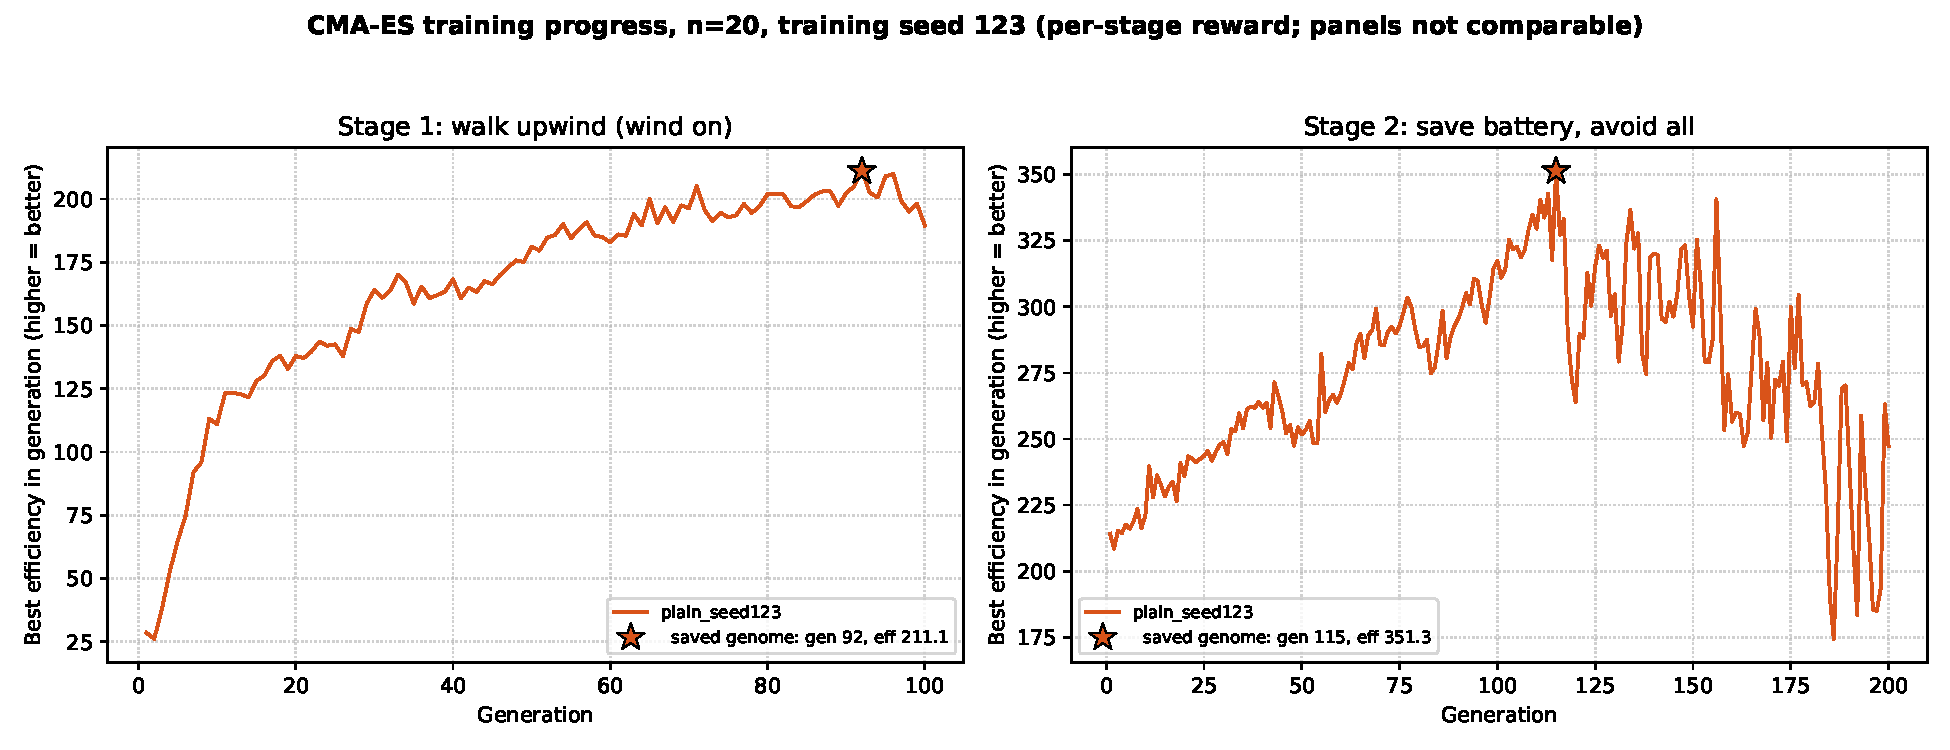
\includegraphics[width=\linewidth]{figures/fitness_curves_plain_seed123_no_clamp}
    \caption[]{Fitness evolution during the two evolutionary stages: fitness of the best candidate in each generation. Stars mark the best candidate ever evaluated, which is the result of the stage.}
    \label{fig:fitness}
\end{figure}


\begin{table}[t]
  \centering
  \caption{Simulation parameters for the baseline controller.}
  \label{tab:baseline_params}
  \begin{tabular}{@{}lll@{}}
    \toprule
    \textbf{Parameter} & \textbf{Description} & \textbf{Value} \\
    \midrule
    $K_{1}$     & MDMC linear gain                           & $0.05~\text{m/s}$ \\
    $K_{2}$     & MDMC angular gain                          & $0.5~\text{rad/s}$ \\
    $\alpha$    & Steepness of potential function            & $2$ \\
    $\epsilon$  & Strength of potential function             & $1$ \\
    $d_{\text{des}}$ & Desired inter–robot distance         & $0.7~\text{m}$ \\
    $D_{\text{p}}$       & Max. interaction range (proximal control)  & $3~\text{m}$ \\
    $K_{\text{goal}}$  & Goal seeking weight                        & $3$ \\
    $k_{\text{align}}$ & Heading-alignment weight & $0$ \\
    $B_0$ & Starting battery & $150$ \\
    \bottomrule
  \end{tabular}
\end{table}


\begin{figure}[t]
  \centering
  \subfloat[\label{fig:scatter_batt_dist}]{
    \begin{minipage}[t]{0.55\textwidth}
      \centering
      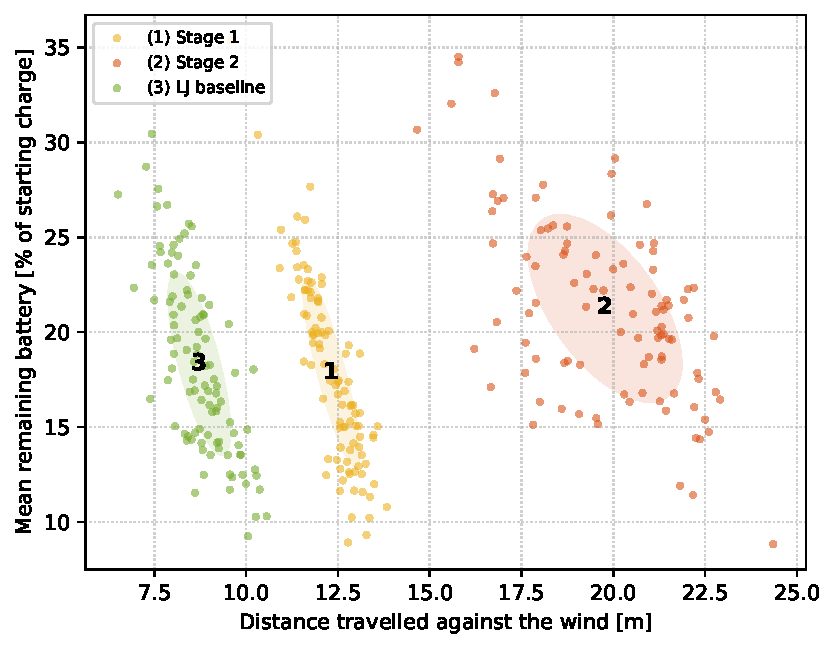
\includegraphics[width=0.98\linewidth]{figures/paper_dist_vs_battery_n20_no_clamp}
    \end{minipage}
  }
  \subfloat[\label{fig:boxplot}]{
    \begin{minipage}[t]{0.40\textwidth}
     \centering
      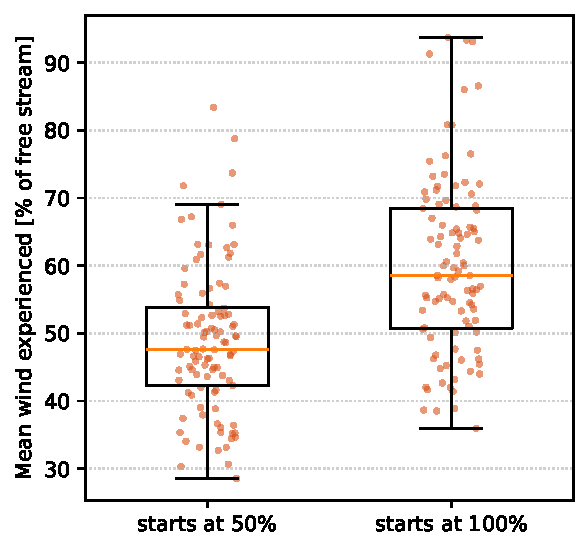
\includegraphics[width=0.95\linewidth]{figures/paper_battery_awareness_boxplot}
    \end{minipage}
  }
\caption{(a) Travelled distance against remaining battery of 100 simulations of 20 robots with the best controller of stage 1 (1), Stage 2 (2), and the baseline (3); ellipses show one standard deviation. (b) Wind speed experienced by the agents initialized at 50\% (left), and 100\% (right) over 100 simulations.}
  \label{fig:joined_scatter_box}
\end{figure}


\begin{table}[t]
\centering
\caption{Performance over 100 simulations of 20 robots (mean $\pm$ standard deviation). ``Both better'' counts the runs in which a controller travels further \emph{and} keeps more battery than the baseline on the same starting configuration. Differences from the baseline are tested with a two-sided Mann--Whitney U test: distance $p < 10^{-33}$ for both controllers; battery $p = 3.3\times10^{-5}$ (Stage 2, higher) and $p = 0.49$ (stage 1, no difference).}
\label{tab:results_main}
{
\begin{tabular}{lccc}
\toprule
\textbf{Controller} & \textbf{Distance [m]} & \textbf{Battery [\%]} & \textbf{Both better} \\
\midrule
Stage 1 & $12.32 \pm 0.74$ & $17.87 \pm 4.87$ & 42/100 \\
Stage 2 & $19.78 \pm 2.05$ & $21.25 \pm 4.85$ & 69/100 \\
Baseline & $8.73 \pm 0.82$ & $18.31 \pm 4.70$ & -- \\
\bottomrule
\end{tabular}}
\end{table}


\begin{table}[t]
\centering
\caption{Results of battery awareness experiment ($p=5.0\times10^{-10}$, $df=198$)}
\begin{tabular}{lccc}
\toprule
\textbf{Experiment} & \textbf{No. of runs} & \textbf{Mean} & \textbf{Standard deviation} \\
\midrule
Agent with 100\% battery & 100 & 60.0 & 13.0 \\
Agent with 50\% battery & 100 & 49.0 & 10.8 \\
\bottomrule
\end{tabular}
\label{tab:results_batt_aware}
\end{table}


\section{Experimental Results}
\label{sec:Exp:Results}

Figure~\ref{fig:fitness} shows the fitness progression of the evolution of the ABCD-rules for a swarm of 20 agents across 300 generations (100 in stage 1 and 200 in Stage 2, as described in Section~\ref{sec:stages}). In Stage 2 the best fitness peaks after 115 generations and declines afterwards. Because we keep the best candidate ever evaluated, the resulting controller comes from this peak. After evolution, we evaluate the best controller obtained after each evolutionary stage and compare it with the baseline of Section~\ref{sec:baseline}. Its robots start with 150 battery units, the native scale of the baseline model, rather than 100. Since the drain per step is the same, they start with $1.5\times$ as much energy; all battery values are reported as a percentage of each controller's own starting charge.

Figure~\ref{fig:scatter_batt_dist}(a) and Table~\ref{tab:results_main} show the main results. Each point in Figure~\ref{fig:scatter_batt_dist} corresponds to one simulation of the best controller from stage 1 (cluster 1), Stage 2 (cluster 2), or the baseline (cluster 3), plotted in terms of distance travelled versus the average battery level of the swarm members at the end of the simulation. Because stage 1 already trains with the wind on and rewards progress against it, the stage-1 controller already travels further than the baseline ($12.3$ vs.\ $8.7$\,m) while keeping a similar amount of battery. Stage 2, which additionally rewards remaining battery and penalises collisions, travels $19.8$\,m, $127\%$ further than the baseline, while also keeping more battery ($21.3\%$ vs.\ $18.3\%$). Both differences are significant (Mann-Whitney U, $p < 10^{-33}$ for distance and $p = 3.3\times10^{-5}$ for battery), and it beats the baseline on both measures at once in 69 of the 100 runs.

The advantage over the baseline depends strongly on the number of robots (Figure~\ref{fig:swarm_size}). The baseline covers about 25\,m with up to 8 robots, but its distance falls steadily as the swarm grows, to 8.8\,m at 20 robots. The evolved controller behaves the other way round: a single robot covers only about 1\,m, and the distance grows with the swarm size to about 20\,m. The controller overtakes the baseline in distance at 12 robots. With 12 or fewer robots it never beats the baseline on distance and battery at the same time in any of 30 runs per swarm size. With 13 robots it does so in 2 of 30 runs, and with 20 robots in 23 of 30. The controllers were evolved with 20 robots only, and they do not transfer to small swarms. Robots learn to rotate constantly when no neighbours are present in Stage 2 of the curriculum as exhibited in Figure~\ref{fig:Debunk_Compass}, thereby wasting battery on these rotations instead of covering more ground.

We argue that the strategies learned in Stage 2 rely primarily on local inter-robot interactions rather than the compass information. We contrast the controllers of stages 1 and 2 by testing them with 1 and 5 robots (Figure~\ref{fig:Debunk_Compass}). The stage 1 controller heads upwind whether it is alone or in a group: a single robot travels about 14\,m, heading straight for the wall and then following it upwind (Figure~\ref{fig:Debunk_Compass}, top left), and five robots move upwind spread out, each on its own path. The Stage 2 controller behaves very differently alone and in a group. A single robot turns in continuous circles and drifts only about a metre (top right), whereas five robots stay together, move upwind and repeatedly loop around one another, changing positions within the group (bottom right). The Stage 2 controller therefore depends on its neighbours to make progress at all: its behaviour is collective, arising from local interactions rather than from the compass alone.

Digging deeper into the effect of the battery-awareness, we compare the effect of two different initial battery levels: 50\% and 100\% and report the results in Figure~\ref{fig:scatter_batt_dist}(b). We measure the percentage of wind exposure in the grid cells the agent visits, $U_{i,j}^\%$, averaged over the simulation time. This captures how much time an agent spends at the front of the swarm, thereby exposing itself to higher wind levels, compared to an agent spending more time in the middle or at the back, thereby experiencing lower wind exposure. Once again, we note that the agents do not have any onboard sensors for wind measurement. We ran 100 simulations with all agents initialized at full charge (100\%) and recorded the average $U_{i,j}^\%$ along the trajectory of a representative agent. We then repeated the experiment, but this time with one agent initialized at half charge (50\%) while all others remained at 100\%. As shown in Figure~\ref{fig:boxplot} and Table \ref{tab:results_batt_aware}, the mean $U_{i,j}^\%$ for a normal agent was 60.0\%, whereas an agent initialized with reduced battery travelled through regions with a lower mean $U_{i,j}^\%$ of 49.0\%. A t-test confirmed the statistical significance of this difference ($t = 6.54$, $p=5.0\times10^{-10}$, $df=198$). This indicates that battery-awareness has allowed the swarm to discover a way to use this information to adapt to unequal battery levels. Thereby allowing the swarm to travel further by shielding the agent with low battery from the wind as it dynamically changes position in response to sensing its own battery being low without the need to communicate with the other agents.

\subsection{Leadership and Position Changes}
\label{sec:leadership_results}




We compute the metrics of Section~\ref{sec:metrics} over 30 simulations of 20 robots for each controller (Table~\ref{tab:leadership} and Figure~\ref{fig:leadership}). The Stage 2 controller changes its front robot about 10 times per minute, almost five times as often as the baseline
(2.1 per minute). Each of these changes lasts at least 1.5\,s, so different robots genuinely take the exposed front position in turn (Figure~\ref{fig:leadership}(a). The raw count of front changes gives the opposite impression: the baseline's front robot changes almost 600 times per simulation, but only about 2\% of those changes persist, because its robots move nearly level with each other and the front identity flickers between them. For the Stage 2 controller, 65\% of the raw changes persist. For the same reason, front occupancy does not separate the controllers at 20 robots (0.84 for Stage 2 against 0.89 for the baseline): the flickering spreads the baseline's front time over many robots. With 10 robots, where the baseline flickers less, the difference is clear (0.90 for the Stage 2 controller against 0.26 for the baseline).

The rotation is not balanced in the sense of Voelkl et al.~\cite{voelkl2015}. The reciprocity between front and back time is negative for the evolved controller ($-0.26$), whereas it is close to zero for the baseline ($0.07$). Robots that spend more time at the front spend less time at the back, so over a whole simulation some robots stay towards the front and others towards the back, even though the front itself changes hands frequently. Neither controller shows a strong turning hierarchy: the leadership entropy is at least 0.97 for both, and the evolved controller's hierarchy is only slightly
steeper than the baseline's (0.63 against 0.55). The evolved behaviour is therefore best described as frequent exchange of the front position without fixed leaders, rather than as a strict rotation through all positions.

\begin{table}[t]
\centering
\caption{Leadership metrics for 20 robots, median [interquartile range] over 30 simulations. All differences from the baseline are significant (Mann-Whitney U, $p < 0.004$).}
\label{tab:leadership}
\small
\begin{tabular}{lcc}
\toprule
\textbf{Metric} & \textbf{Stage 2} & \textbf{Baseline} \\
\midrule
Front changes per minute & 9.9 [9.5, 10.2] & 2.1 [1.7, 2.5] \\
Raw changes that persist [\%] & 65 [57, 68] & 2.1 [1.8, 2.6] \\
Front occupancy entropy & 0.84 [0.81, 0.88] & 0.89 [0.88, 0.91] \\
Reciprocity $r$ & $-0.26$ [$-0.34$, $-0.21$] & 0.07 [$-0.04$, 0.19] \\
Hierarchy entropy & 0.98 [0.97, 0.98] & 0.99 [0.99, 0.99] \\
Hierarchy steepness & 0.63 [0.55, 0.69] & 0.55 [0.50, 0.59] \\
\bottomrule
\end{tabular}
\end{table}

\begin{figure}[t]
  \centering
  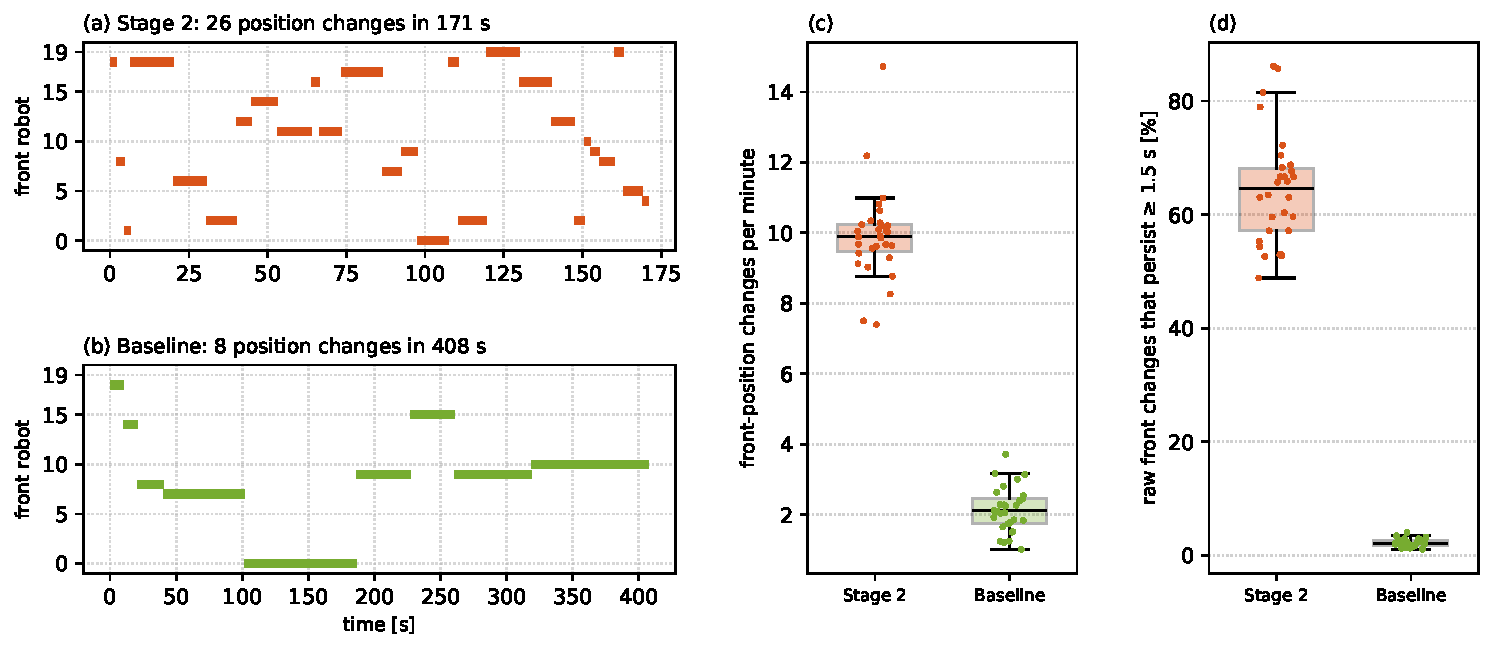
\includegraphics[width=\linewidth]{figures/paper_leadership_n20_no_clamp}
  \caption{Front-position changes with 20 robots. (a, b) Which robot is at the front over time in one simulation, after discarding spells shorter than 1.5\,s, for the stage-2 controller and the baseline; note the different time axes. (c) Front-position changes per minute and (d) share of raw front changes that persist for at least 1.5\,s, over 30 simulations per controller.}
  \label{fig:leadership}
\end{figure}

\subsection{Real-Robot Experiments}
\label{sec:hardware_results}

In simulation, the controller does not outperform the baseline in swarms as small as those we can run on real robots (Figure~\ref{fig:swarm_size}). \rev{The real-robot experiments therefore test whether the evolved behaviour transfers from simulation to hardware, not whether it beats the baseline.} \rev{Since the wind and the battery remain simulated on hardware, we focus on the turn-taking behaviour and compare each controller with 30 simulations of the same controller with seven robots, using the protocol of Table~\ref{tab:leadership}.}

\rev{We compute the leadership metrics of Section~\ref{sec:metrics} on the longest window of each trial with valid position estimates for all seven robots (Section~\ref{sec:hardware_setup}).} \rev{This window covers the whole trial in 22 of the 30 baseline trials and in 20 of the 30 Stage~2 trials; its median length is 59\,s for both.}

\rev{Tables~\ref{tab:leadership_hardware_hw} and \ref{tab:leadership_hardware_sim} and Figure~\ref{fig:hardware_lighthouse} show the results.} \rev{The main simulation result transfers to hardware: the Stage~2 controller shares the exposed front among the robots much more evenly than the baseline.} \rev{Its front-occupancy entropy is $0.75$ against $0.33$ for the baseline ($p < 10^{-9}$), as in simulation ($0.88$ against $0.16$).} \rev{The front changes hands $7.4$ times per minute with the Stage~2 controller, as often as in simulation ($8.2$, $p = 0.41$) and more often than with the baseline ($5.1$, $p = 0.002$).} \rev{The baseline changes its front robot more often on hardware than in simulation ($5.1$ against $2.3$ per minute), but a smaller share of its raw front changes persist ($18\%$ against $33\%$ in simulation; $30\%$ against $48\%$ for Stage~2).} \rev{On hardware, noise in the positions and imperfect execution make robots that are nearly level swap ranks more often, and the persistence filter removes this flicker only partly.} \rev{This also raises the baseline's front-occupancy entropy above its simulated value ($0.33$ against $0.16$), while Stage~2's is lower than in simulation ($0.75$ against $0.88$).} \rev{The gap between the two controllers therefore narrows on hardware but remains large.}

\rev{As in simulation, the reciprocity between front and back time is negative for both controllers: robots that spend more time at the front spend less time at the back.} \rev{For Stage~2 it matches the simulated value ($-0.46$ against $-0.50$, $p = 0.61$), and it is more negative than the baseline's ($-0.33$, $p = 0.027$), so the evolved controller does not produce more reciprocal turn-taking than the baseline on hardware either.} \rev{Neither the hierarchy entropy ($0.93$ and $0.94$) nor the steepness ($0.79$ and $0.76$) separates the controllers on hardware ($p \geq 0.12$), as in simulation.}

\rev{The two controllers also move differently.} \rev{In 60\,s the baseline travels $5.5 \pm 0.1$\,m upwind as a closely aligned group.} \rev{Stage~2 travels $3.4 \pm 0.6$\,m: its robots stay close together (mean nearest-neighbour distance $0.35$\,m) and keep looping around each other.} \rev{The brake (Equation~\ref{eq:brake}) slows them in $32\%$ of the robot steps, and robots touch (centres closer than $0.12$\,m) during $1.2\%$ of the time.} \rev{Their mean wind exposure is $74\%$ against $64\%$ for the baseline, but since they also move less, they end the trial with slightly more virtual battery ($78\%$ against $76\%$).} \rev{The baseline's lead in distance matches the simulation at this swarm size (Figure~\ref{fig:swarm_size}).}

\rev{Overall, the evolved controller shares the exposed front among more robots than the baseline on real robots as in simulation, and changes its front robot as often as in simulation.} \rev{As in simulation, this exchange is not a balanced rotation in the sense of Voelkl et al.~\cite{voelkl2015}.}

\begin{table}[t]
\centering\color{red}
\caption{Leadership metrics on the real robots ($n=7$), median [interquartile range] over 30 trials per controller, computed on each trial's longest window with valid positions (Section~\ref{sec:hardware_results}). Difference from the baseline (Mann-Whitney U): $^{ns}p\geq0.05$, $^{*}p<0.05$, $^{**}p<0.01$, $^{***}p<0.001$. Compare against Table~\ref{tab:leadership_hardware_sim}.}
\label{tab:leadership_hardware_hw}
\small
\begin{tabular}{lcc}
\toprule
\textbf{Metric} & \textbf{Stage 2} & \textbf{Baseline} \\
\midrule
Front changes per minute & 7.4 [6.2, 10.3]$^{**}$ & 5.1 [3.1, 7.2] \\
Raw changes that persist [\%] & 30 [24, 42]$^{***}$ & 18 [13, 23] \\
Front occupancy entropy & 0.75 [0.62, 0.82]$^{***}$ & 0.33 [0.28, 0.36] \\
Reciprocity $r$ & $-0.46$ [$-0.59$, $-0.27$]$^{*}$ & $-0.33$ [$-0.37$, $-0.27$] \\
Hierarchy entropy & 0.93 [0.90, 0.95]$^{ns}$ & 0.94 [0.92, 0.96] \\
Hierarchy steepness & 0.79 [0.75, 0.89]$^{ns}$ & 0.76 [0.67, 0.84] \\
\bottomrule
\end{tabular}
\end{table}

\begin{table}[t]
\centering\color{red}
\caption{As Table~\ref{tab:leadership_hardware_hw}, for the matched simulations: 30 simulations per controller with seven robots, with the same methodology as Table~\ref{tab:leadership}.}
\label{tab:leadership_hardware_sim}
\small
\begin{tabular}{lcc}
\toprule
\textbf{Metric} & \textbf{Stage 2} & \textbf{Baseline} \\
\midrule
Front changes per minute & 8.2 [7.5, 9.7]$^{***}$ & 2.3 [0.6, 7.3] \\
Raw changes that persist [\%] & 48 [43, 55]$^{***}$ & 33 [23, 42] \\
Front occupancy entropy & 0.88 [0.86, 0.95]$^{***}$ & 0.16 [0.09, 0.34] \\
Reciprocity $r$ & $-0.50$ [$-0.59$, $-0.35$]$^{***}$ & $-0.20$ [$-0.30$, $-0.18$] \\
Hierarchy entropy & 0.94 [0.93, 0.96]$^{ns}$ & 0.92 [0.89, 0.95] \\
Hierarchy steepness & 0.79 [0.70, 0.81]$^{ns}$ & 0.82 [0.75, 0.87] \\
\bottomrule
\end{tabular}
\end{table}

\begin{figure}[t]
  \centering\color{red}
  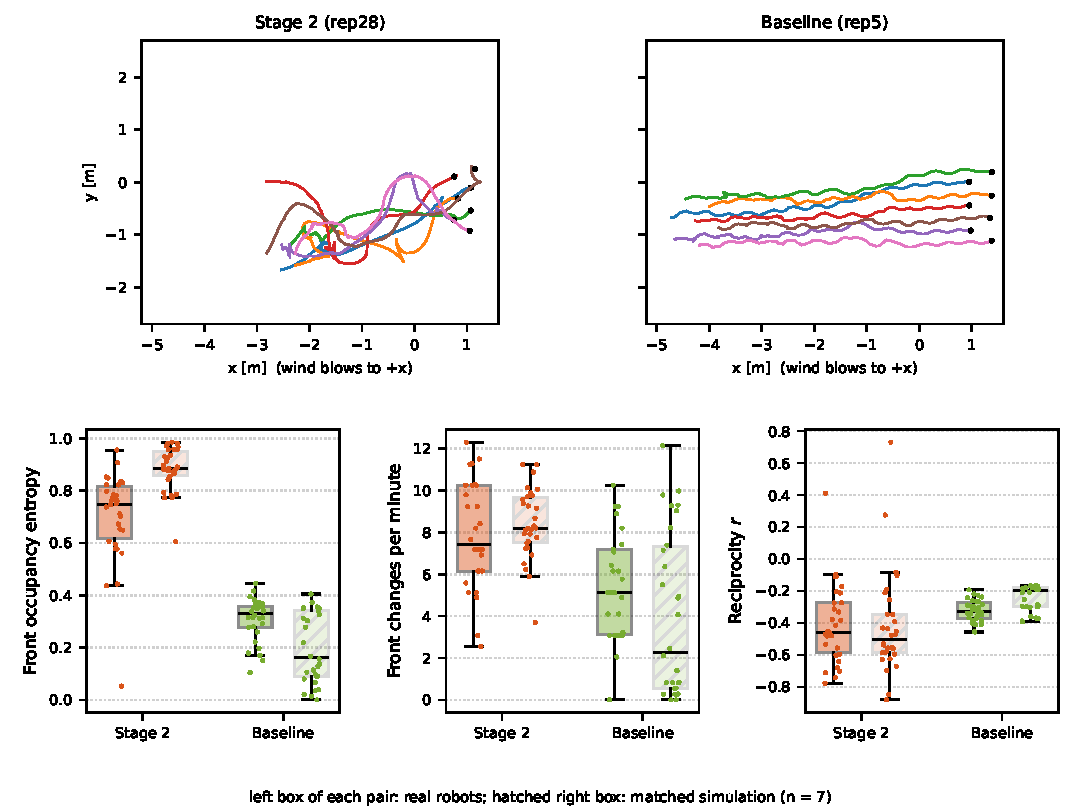
\includegraphics[width=\linewidth]{figures/hardware_lighthouse_no_clamp}
  \caption{Real robots ($n=7$). Top: trajectories in one trial per controller (the trial with the median front-occupancy entropy), over the window used for the metrics; dots mark the start positions and the wind blows towards $+x$. Bottom: front-occupancy entropy, front changes per minute and reciprocity for every real trial (left box of each pair) and for the 30 matched simulations with seven robots (hatched right box).}
  \label{fig:hardware_lighthouse}
\end{figure}

\begin{figure}[t]
  \centering
  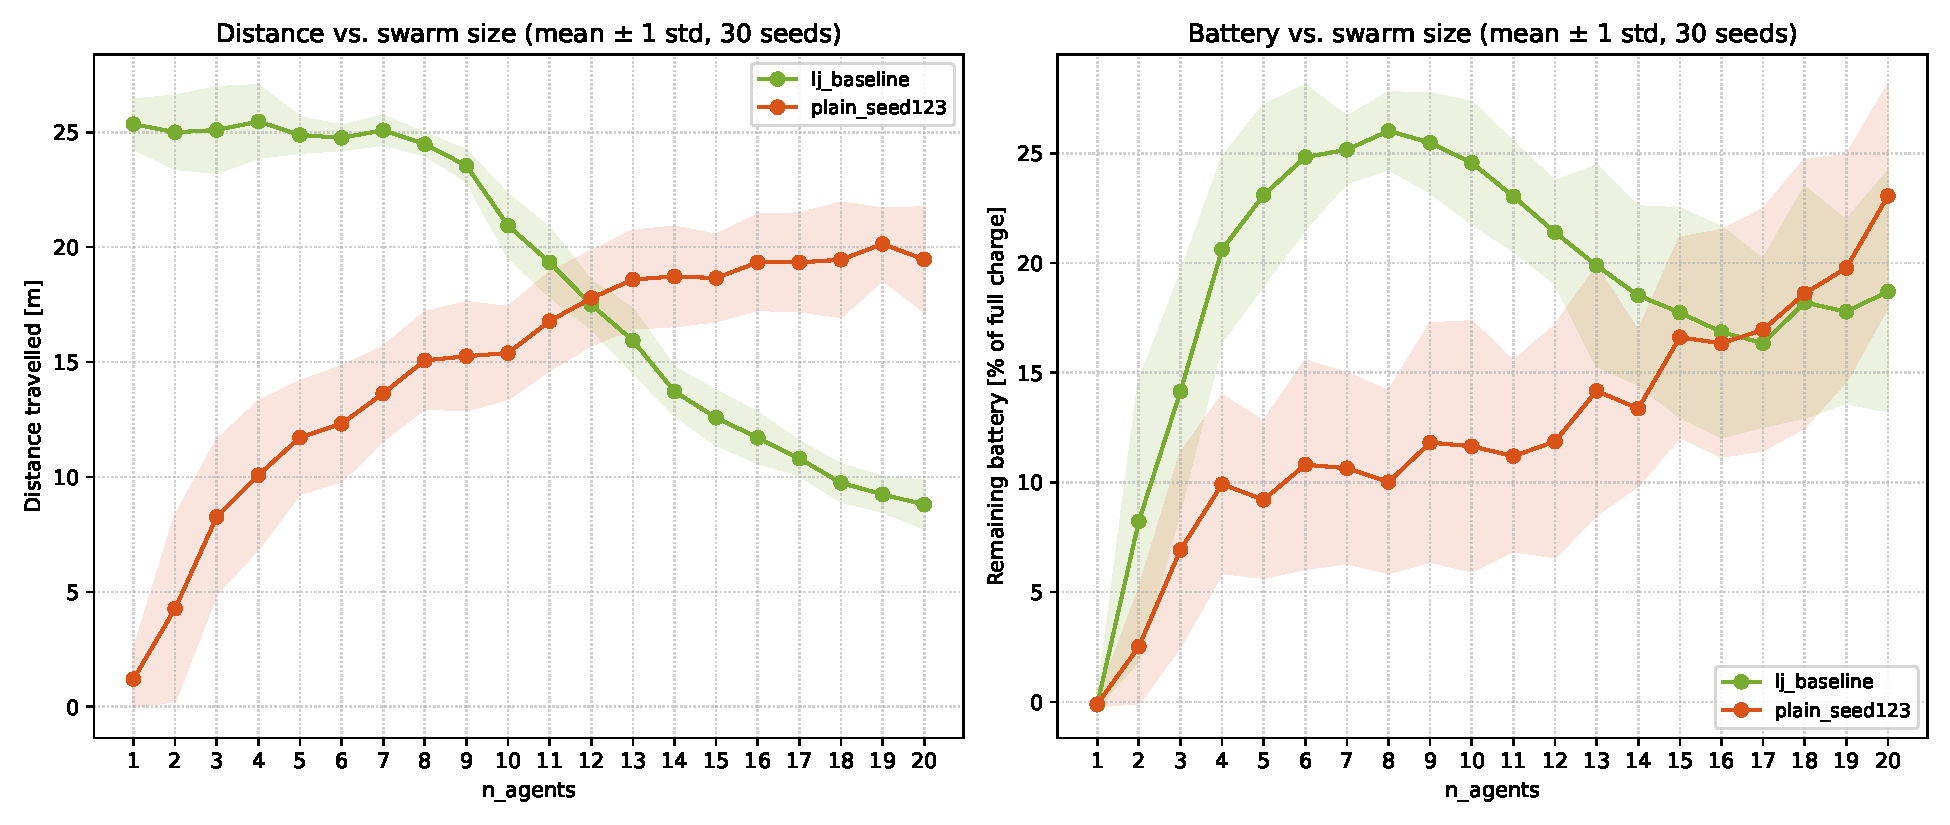
\includegraphics[width=\linewidth]{figures/n_agents_sweep_distance_battery_plain_seed123_no_clamp}
  \caption{Distance (left) and remaining battery (right) against swarm size, mean $\pm$ one standard deviation over 30 simulations per size, for the baseline (green) and the Stage~2 controller (orange). The Stage~2 controller was evolved with 20 robots.}
  \label{fig:swarm_size}
\end{figure}


\begin{figure}[t]
  \centering
  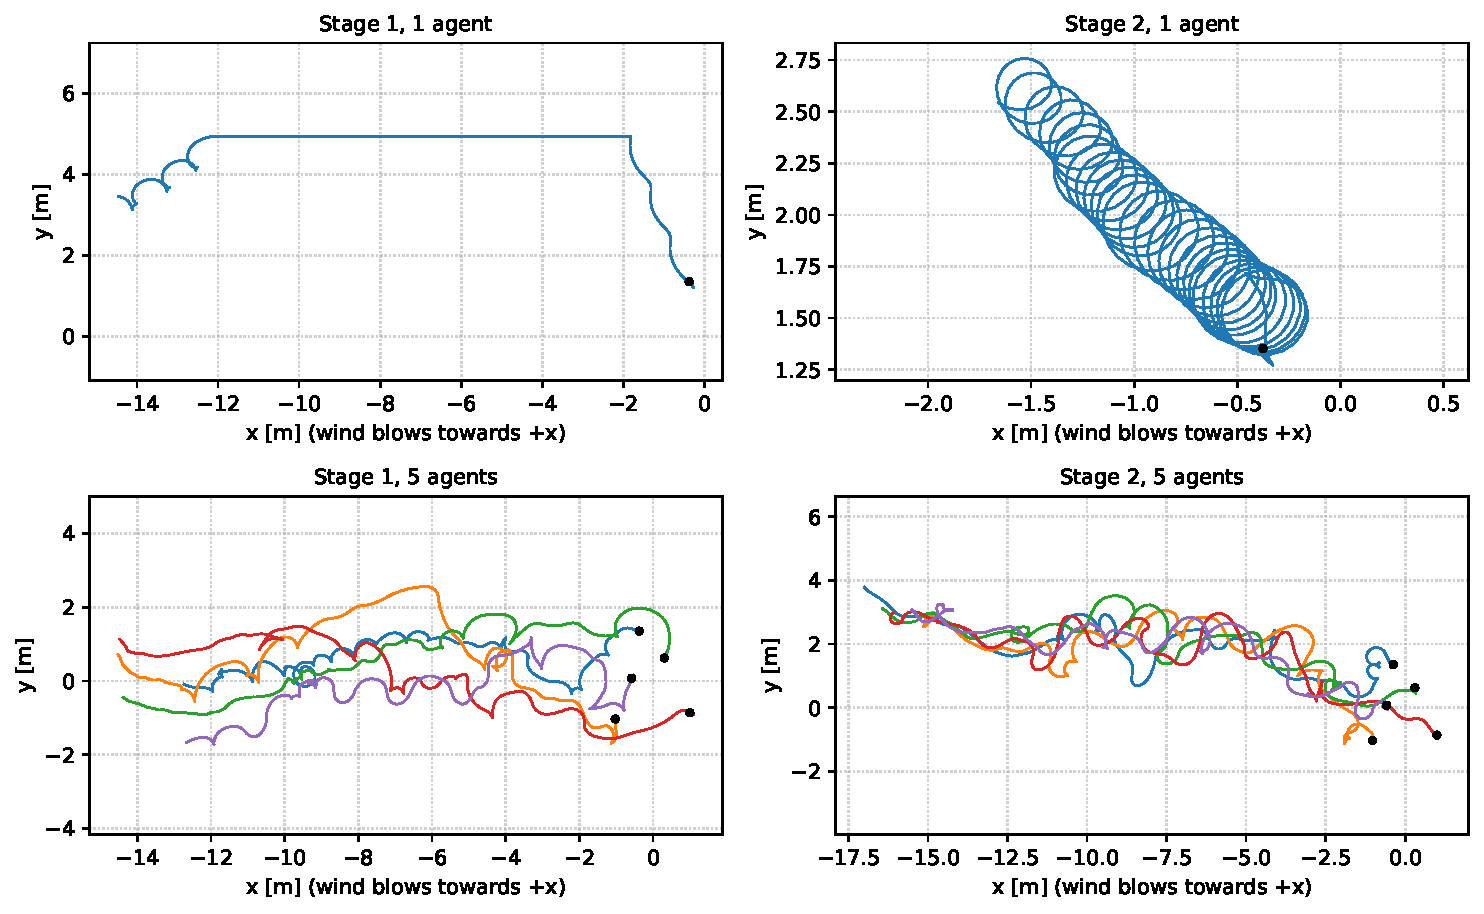
\includegraphics[width=\linewidth]{figures/paper_trajectories_stage1_vs_stage2}
  \caption{Trajectories of the best controller from stage 1 (left) and Stage 2 (right) with one (top) and five (bottom) robots; black dots mark the starting positions. Note the different axis scales in the top-right panel.}
  \label{fig:Debunk_Compass}
\end{figure}

%The source code and the supplementary video are available in the Zenodo repository at \url{https://doi.org/10.5281/zenodo.18602800}.
%\todo[inline]{Update the Zenodo release (code, controllers, supplementary video) to the two-stage version and replace this link.}



\section{Conclusion}
\label{sec:Conclusion}

Taking inspiration from natural collectives such as bird flocks, we have investigated whether battery-awareness combined with neighbour sensing is sufficient for a swarm of simulated agents and real robots to discover the turn-taking strategy that those natural flocks often employ to reduce the effect of wind exposure on the energy level. Our results show that this strategy indeed emerges without including turn-taking or a wind sensor in the fitness function.  With 20 robots, the resulting controller travelled $127\%$ further on average than a flocking baseline while also keeping more battery. This advantage only appears in large swarms: with 12 or fewer robots the baseline performs better, and a single robot with the evolved controller hardly travels any distance along the x-axis but moves in circles. In the evolved swarm the front position changes hands about ten times per minute, almost five times as often as in the baseline, although robots do not cycle evenly between front and back. \rev{On seven real robots, the evolved controller spreads the time at the exposed front over more robots than the baseline, as in simulation, and changes its front robot as often as it does in simulation.} \rev{As in simulation, the exchange is not balanced: robots that lead more trail less.} While these results are promising, they are heavily dependent on the swarm size. Future work should investigate how this limitation can be mitigated. In addition, a comparison of the battery-awareness with other information sources such as an actual wind sensor should be undertaken. Further hardware validation in a bigger arena that would fit a bigger swarm size would also be beneficial to see if the patterns reported for the hardware would also hold at larger swarm sizes.


\begin{credits}

\subsubsection{\ackname}
This work is supported in part by the NYUAD Center for Artificial Intelligence and Robotics (CAIR), funded by Tamkeen under the NYUAD Research Institute Award CG010, and by the NYUAD Center for Interdisciplinary Data Science \& AI (CIDSAI), funded by Tamkeen under the NYUAD Research Institute Award CG016.

\subsubsection{\discintname}
The authors declare they have no competing interests.

\end{credits}




\bibliographystyle{splncs04}
\bibliography{mybibliography}

\end{document}
